%!TEX root=../../template.tex
\section{The Experiment}%
\label{sec:the_experiment}

As stated in this chapter's introductory notes, this thesis main body of
work revolves around two base assumptions, our hypothesis. The first
one, about the information capturing by the idealised system, was
addressed in Subsection~\ref{sub:discretisation}. The second, more
physical in nature, is the subject matter of this section. Our
hypothesis states that the light absorption between points $A$ and $B$
(let's call it $A_{AB}$) should be equal to the difference of the
absorptions in $A$ and $B$. We can write this, in a \emph{Lambertian}
manner as in Equation~\ref{eq:lambertian_hypothesis}.

\begin{equation}
    \label{eq:lambertian_hypothesis}
    I_B = I_A \cdot \exp \bigg[-AB \cdot \sum_i \sigma_{ABi} \cdot
    c_{ABi}\bigg]
\end{equation}

This is to say that the light intensity reaching point $B$ is given by
the intensity reaching $A$, exponentially decreased by the absorbers at
interval $AB$. The intensities at $A$ and $B$ are written as in
Equation~\ref{eq:intensityAtAAndB}.

\begin{equation}
    \begin{aligned}
        \label{eq:intensityAtAAndB}
        I_B = I_0 \cdot \exp \bigg[ -L_B \cdot \sum_i \sigma_{Bi} \cdot
        c_{Bi} \bigg]\\
        I_A = I_0 \cdot \exp \bigg[ -L_A \cdot \sum_i \sigma_{Ai} \cdot
        c_{Ai} \bigg]
    \end{aligned}
\end{equation}

If we join all this information in the same expression, the equation is
transformed into its final form, presented in
Equation~\ref{eq:hypothesis_final_form}.

\begin{equation}
    \small
    \label{eq:hypothesis_final_form}
    I_0 \cdot \exp \bigg[ -L_B \cdot \sum_i \sigma_{Bi} \cdot
            c_{Bi} \bigg] = I_0 \cdot \exp \bigg[ -L_A \cdot \sum_i \sigma_{Ai} \cdot
            c_{Ai} \bigg] \cdot \bigg[-AB \cdot \sum_i \sigma_{ABi} \cdot
            c_{ABi}\bigg]
\end{equation}

Equation~\ref{eq:hypothesis_final_form} can be greatly simplified: we
take the natural logarithm of both sides and we state that $\sum_i
\sigma_{Xi} \cdot c_{Xi} = S_i$. These operations result in the
simplified form of Equation~\ref{eq:final_form_simplified}.

\begin{equation}
    \label{eq:final_form_simplified}
    L_B \cdot S_B = L_A \cdot S_A + L_{AB} \cdot S_{AB}
\end{equation}

Now, $L_X \cdot S_X$ can be thought of as the wavelength dependent light
absorption in path $X$. In this case, the wavelength interval is always
the same. We can therefore conclude that, theoretically, our
hypothesis is valid: light absorption between points $A$ and $B$ can be
expressed in terms of the absorption on both these points and
corresponds to their difference.

Although mathematically this seems clear-cut, in the real world things
can become more problematic, since we have to deal with the
imperfections that characterise a real physical system. Noise,
instrumental limitations, adverse environmental effects, etc.. The
experiment we describe in the next few paragraphs aimed at determining
target trace gas concentration in a set analysis field. This field is
dimension-wise compatible with those that would be employed in the final
working system. This experiment is represented in
Figure~\ref{fig:experiment_map}.

\begin{figure}[htpb]
    \centering
    \includegraphics[width=0.8\linewidth]{img/png/experimentMap.png}
    \caption{Location of observer points for the physical experiment.}
    \label{fig:experiment_map}
\end{figure}

The goal of the experiment was to compare passive and active \gls{DOAS}
measurements performed with a very short time difference between them.
The passive measurement would employ the same acquisition strategy as
the drone is expected to use. This comparison will be used to test our
second hypothesis.

Finding two appropriate experiment sites proved to be the first
difficulty: both telescopes should see sky on the back of the other
telescope. Otherwise, the contribution from the terrain's reflection
would have to be taken into account and the experiment conditions would
be very different from the ones the drone will have. There are not many
site pairs that provide this, and most of the ones that exist are
private and authorisations are not easy to obtain. In the end, we
managed to run the experiment in the facilities of \emph{\gls{iep}} and
the \emph{Cristo-Rei} sanctuary, near our own base. 

\subsection{Protocol and conduction}%
\label{sub:protocol_and_conduction}

The experiment involved two different optical assemblies, which are
summarised in Table~\ref{tab:assemblies}. Both assemblies play two
roles, which reflect the comparison between active and passive that is
the entire aim of the test. To simplify, we will address the two as West
Bank and East Bank. The West Bank is, as the name implies, the assembly
that is placed further West, i.e., the one that is installed on
\gls{iep}'s roof. By exclusion, the East Bank assembly is the one placed
on the sanctuary. The West Bank assembly is comprised of a telescope and
tripod, a spectrometer (with the necessary fibre optics attached) and a
laptop. 

The East Bank assembly has exactly the same parts, but in addition to
them, it features a hand-held torch that sports an XHP50.2 CREE LED. The
manufacturer states that this torch is capable of illuminating by itself
up to a distance of 300 m and produces luminous flux of at least 1500
lm. By fitting this torch on the telescope's eyepiece channel, we are
able to further collimate the light that it produces, making it reach
much further distances than originally stated, and being easily picked
up by the other telescope. This is plain to see in
Figure~\ref{fig:light_at_the_distance}. The light spectrum that pertains
to the CREE LED in use is published in this device's datasheet, and
presented in Figure~\ref{fig:cree_spectrum}, which largely corroborates
the spectrum in Figure~\ref{fig:measured_led_spectrum}, taken by the
same spectrometers that were used in the experiment, at a distance of
approximately 50 m from the torchlight. 

\begin{figure}[htpb]
    \begin{minipage}{.45\textwidth}
        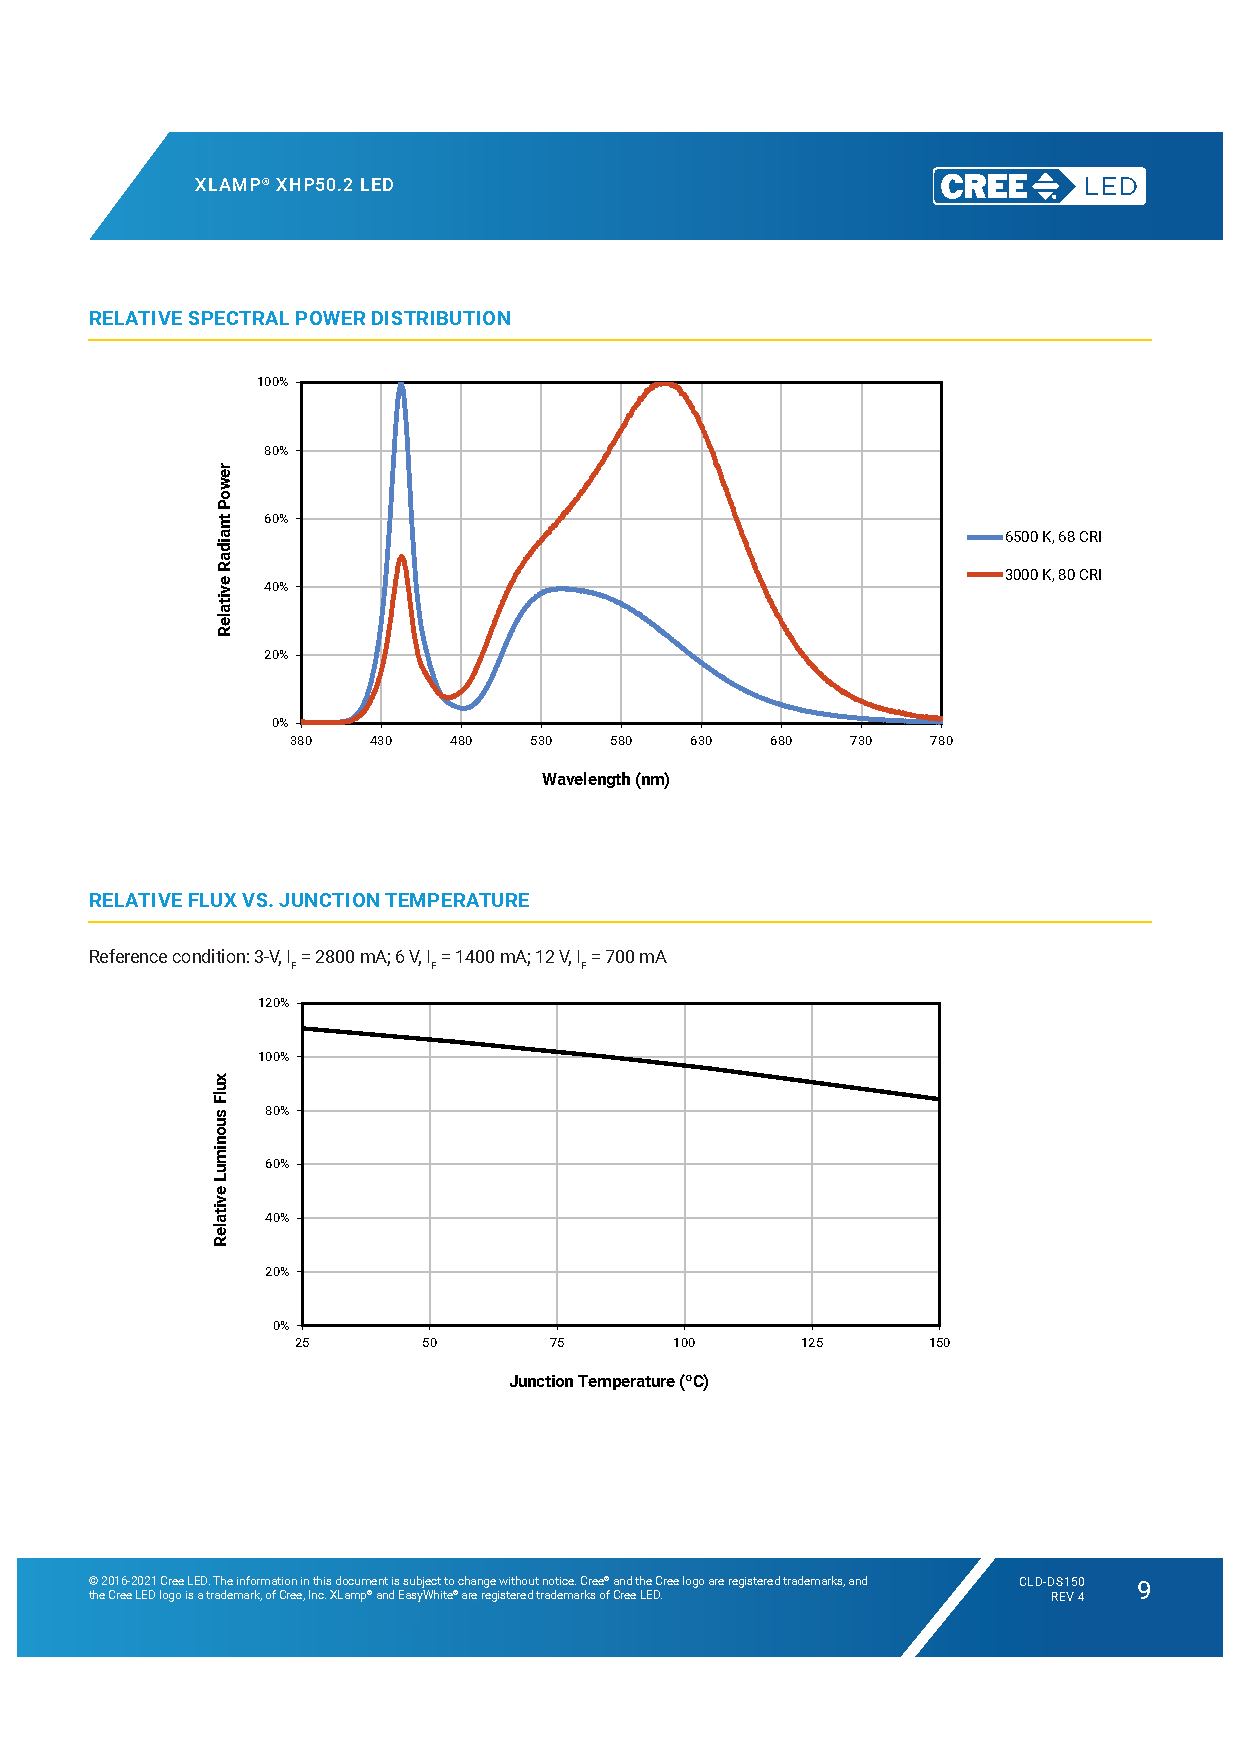
\includegraphics[trim=3cm 15cm 5cm 6cm, % ...
            clip, width=\textwidth]{img/pdf/cree_datasheet.pdf}
        \caption{Published spectrum of the CREE XHP50.2 LED
        light. The LED that was used in this
        experiment corresponds to the blue line~\cite{CREE2021}.}
        \label{fig:cree_spectrum}
    \end{minipage}
    \hfill
    \begin{minipage}{.45\textwidth}
        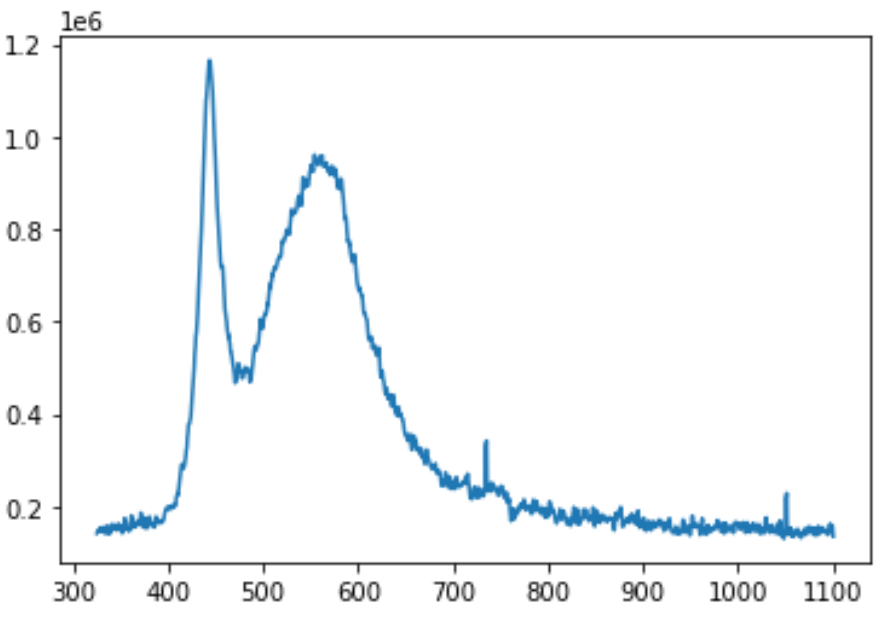
\includegraphics[width=\textwidth]{img/png/measured_led_spectrum.png}
        \caption{Spectrum measured with the experiment spectrometers, at
        a distance of approximately 50 m from the torchlight.}
        \label{fig:measured_led_spectrum}
    \end{minipage}
\end{figure}

\begin{table}[htpb]
    \centering
    \caption{Summary table for the two experiment assemblies. Note the
    difference in terms of material, due to the two different roles both
    assemblies play during the experiment. This is translated into not
    having the need of an artificial light source in the West Bank's
    assembly.}
    \label{tab:assemblies}
    \resizebox{\textwidth}{!}{%
        \begin{tabular}{@{}lll@{}}
            \toprule
            \textbf{} & \textbf{West Bank} & \textbf{East Bank} \\ \midrule
            \textbf{Spectrometer} & Avantes USB 2048 channels & Avantes USB 2048 channels \\
            \textbf{Telescope} & Meade ET90 & Meade ET90 \\
            \textbf{Artificial Light Source} & N/A & Goobay CREE XHP50.2 torch \\
            \textbf{Laptop} & Windows 10 laptop & Windows 10 laptop \\
            \textbf{Software} & AvaSoft 8.11 & AvaSoft 8.11 \\ \bottomrule
        \end{tabular}%
    }
\end{table}

The experiment itself is scheduled to start at around 06:00 A.M.. It
consists in capturing spectral measurements in both modes (active and
passive) periodically, with the least amount of time possible between
measurements in the same capture. In this case, I am calling capture to
a particular group of actions that are defined in
Table~\ref{tab:actions}. Captures are defined according to the time at
which they are run, and are summarised in Table~\ref{tab:captures}.
Closing time for this experiment was set on 11:00 A.M.. This time window
ensures measurements are taken during sunrise and until after the
morning rush hour is over.

\begin{table}[htpb]
    \centering
    \small
    \caption{Actions are the indivisible unit upon which each capture is
    built. The prescribed actions for this experiment are described in
    this table.}
    \label{tab:actions}
    \begin{tabularx}{\textwidth}{cXX}
        \toprule
        \textbf{Action ID} & \textbf{Action} & \textbf{Description} \\ \midrule
        A & Active trace gas concentration determination & With the two
        telescopes facing each other, we collect spectra for two minutes
        with the light source turned off and another 2 min with the light
        source turned on. \\
        \midrule
        B & Passive trace gas concentration determination & With the two
        telescopes aligned and approximately facing West, we collect spectra
        for 2 minutes. \\
        \midrule
        C & Passive reference collection & The West telescope points upwards
        and collects data for 2 minutes. \\ \bottomrule
    \end{tabularx}
\end{table}

\begin{table}[htpb]
    \centering
    \caption{Captures are particular sets of actions that are conducted
    according to a specific order, depending on the time of day on which
    the capture is run. This table describes the prescribed captures on
    which this experiment consisted.}
    \label{tab:captures}
    \begin{tabular}{@{}ccc@{}}
        \toprule
        \textbf{Time Frame} & \textbf{Period} & \textbf{Action} \\
        \midrule
        05:00 - Sunrise & 15 minutes & A \\
        Sunrise & Once & C \\
        Sunrise - 11:00 & 15 minutes & A and B\\
        \bottomrule
    \end{tabular}
\end{table}

As displayed in Table~\ref{tab:assemblies}, the spectrometers are both
the same model, manufactured by Avantes and with 2048 channels, powered
through the same \gls{usb} cable that is used for data transfer. The
spectra are acquired through Avantes' own collection software, AvaSoft
8. The spectrometer are configured to have an integration time of 20ms
and immediately store every measurement on an \gls{ascii} file. With the
kind of lighting conditions that we are dealing with, this integration
time allows us not to worry about saturation. However, to build usable
spectra we need to sum the collected files. This is valid because given
the very little time it takes to make a measurement (2 minutes), the sun
can be considered a constant light source, and therefore
we can consider the photons to have a Poissonian statistic
distribution~\cite{Fox2006}.

\subsection{First Run}%
\label{sub:experiment_first_run}

The first attempt at running this experiment took place on June
7\textsuperscript{th} 2021. Weather conditions were optimal for this
kind of measurement, with no wind, clear sky and very low optical
density, as can is testified by Figure~\ref{fig:light_at_the_distance}.
The experiment started with a small delay, caused by a problem on the
charger of the East bank laptop. Besides this delay, this was not a
problem for the experiment itself. It was the other laptop's battery
that did not hold enough charge for the experiment to reach its
determined end, and there was no means to charge it on \gls{iep}'s roof.
Given this circumstance, we were able to retrieve spectral measurements
from around 06:20 A.M. to 08:20 A.M., in a total of 6 measurements which
are produced in Table~\ref{tab:experiment_measurements}.

\begin{figure}[htpb]
    \centering
    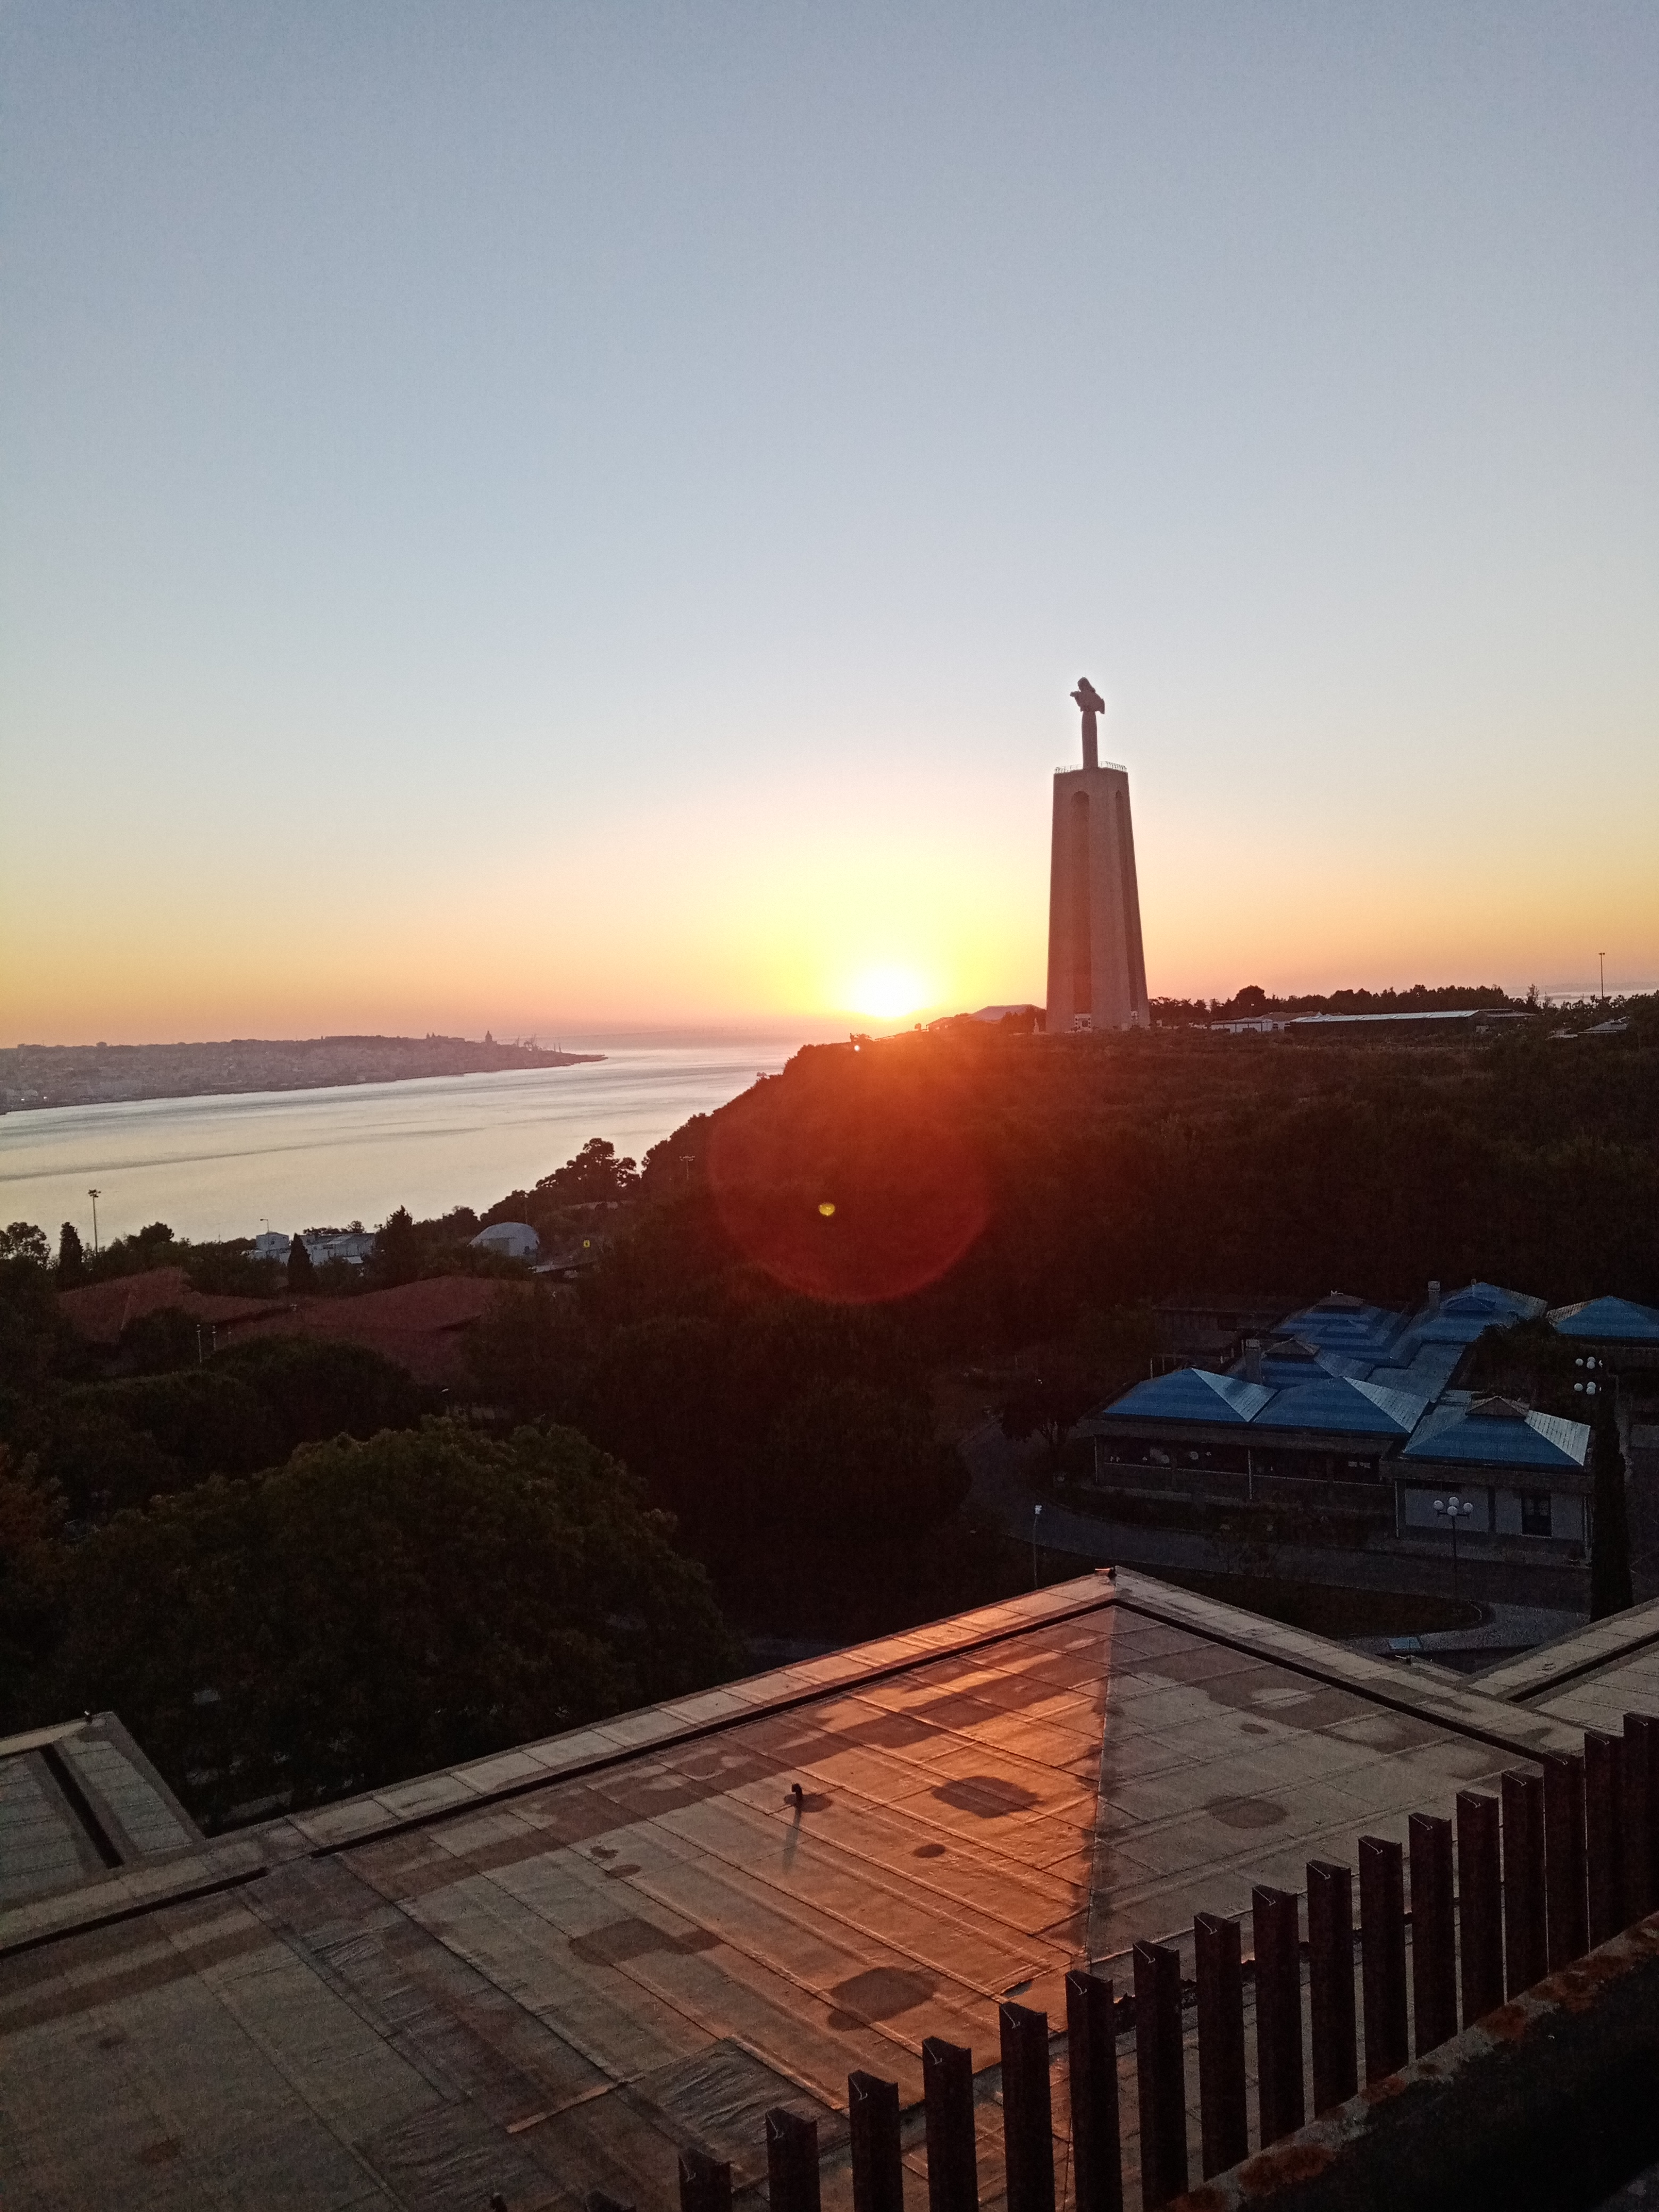
\includegraphics[width=0.8\linewidth]{img/jpg/experiment1/light_at_the_distance1.jpg}
    \caption{View from West Bank assembly at sunrise during the first
    run of the experiment. Note that even with the sun appearing in the
    back, the light from the torch is perfectly visible at this distance.}
    \label{fig:light_at_the_distance}
\end{figure}


\begin{table}[htpb]
    \centering
    \caption{First run: measurement table.}
    \label{tab:experiment_measurements}
    \resizebox{\textwidth}{!}{%
        \begin{tabular}{@{}lllll@{}}
            \toprule
            \textbf{\#} & \textbf{Passive meas.} & \textbf{Passive ref.} & \textbf{Active mean.} & \textbf{Active ref.} \\ \midrule
            1 & 06:20 & 06:23 & 06:15 & -- \\
            2 & 06:46 & 06:50 & 06:41 & -- \\
            3 & 07:04 & 07:07 & 07:00 & -- \\
            4 & 07:25 & 07:27 & 07:21 & -- \\
            5 & 07:48 & 07:50 & 07:45 & -- \\
            6 & 08:10 & 08:12 & 08:06 & 08:08 \\ \bottomrule
        \end{tabular}%
    }
\end{table}

On the one hand, it is clear from
Table~\ref{tab:experiment_measurements} that we do not have data on the
active baseline spectra~\footnote{In this case, the baseline spectrum is
one taken in the exact same direction and approximately
simultaneously, with the light turned off to allow removal of solar
contribution.} (likely due to some operation error); on the other hand,
we have too few data points to make any claim of validation or
refutation of the principle we were to measure. It was thus clear that
another run was necessary to get satisfactory results.

Although the collected data did not allow to make any claims whatsoever,
they were of good individual quality and allowed for a partial analysis
to be run, namely the passive \gls{DOAS} side. Using the first
measurement as the reference spectrum, it was possible to calculate the
\gls{no2} concentration. The fits that generated these concentration
values are presented in Figure~\ref{fig:exp1_fit_west} and
Figure~\ref{fig:exp1_fit_east}, respectively, for the West and East
assemblies. The molecular density values for \gls{no2} are presented in
Figure~\ref{fig:exp1_no2_density}. The \gls{DOAS} parameters for this
run of the experiment are presented in
Table~\ref{tab:doas_parameters_exp1}

\begin{sidewaysfigure}[htpb]
    \centering
    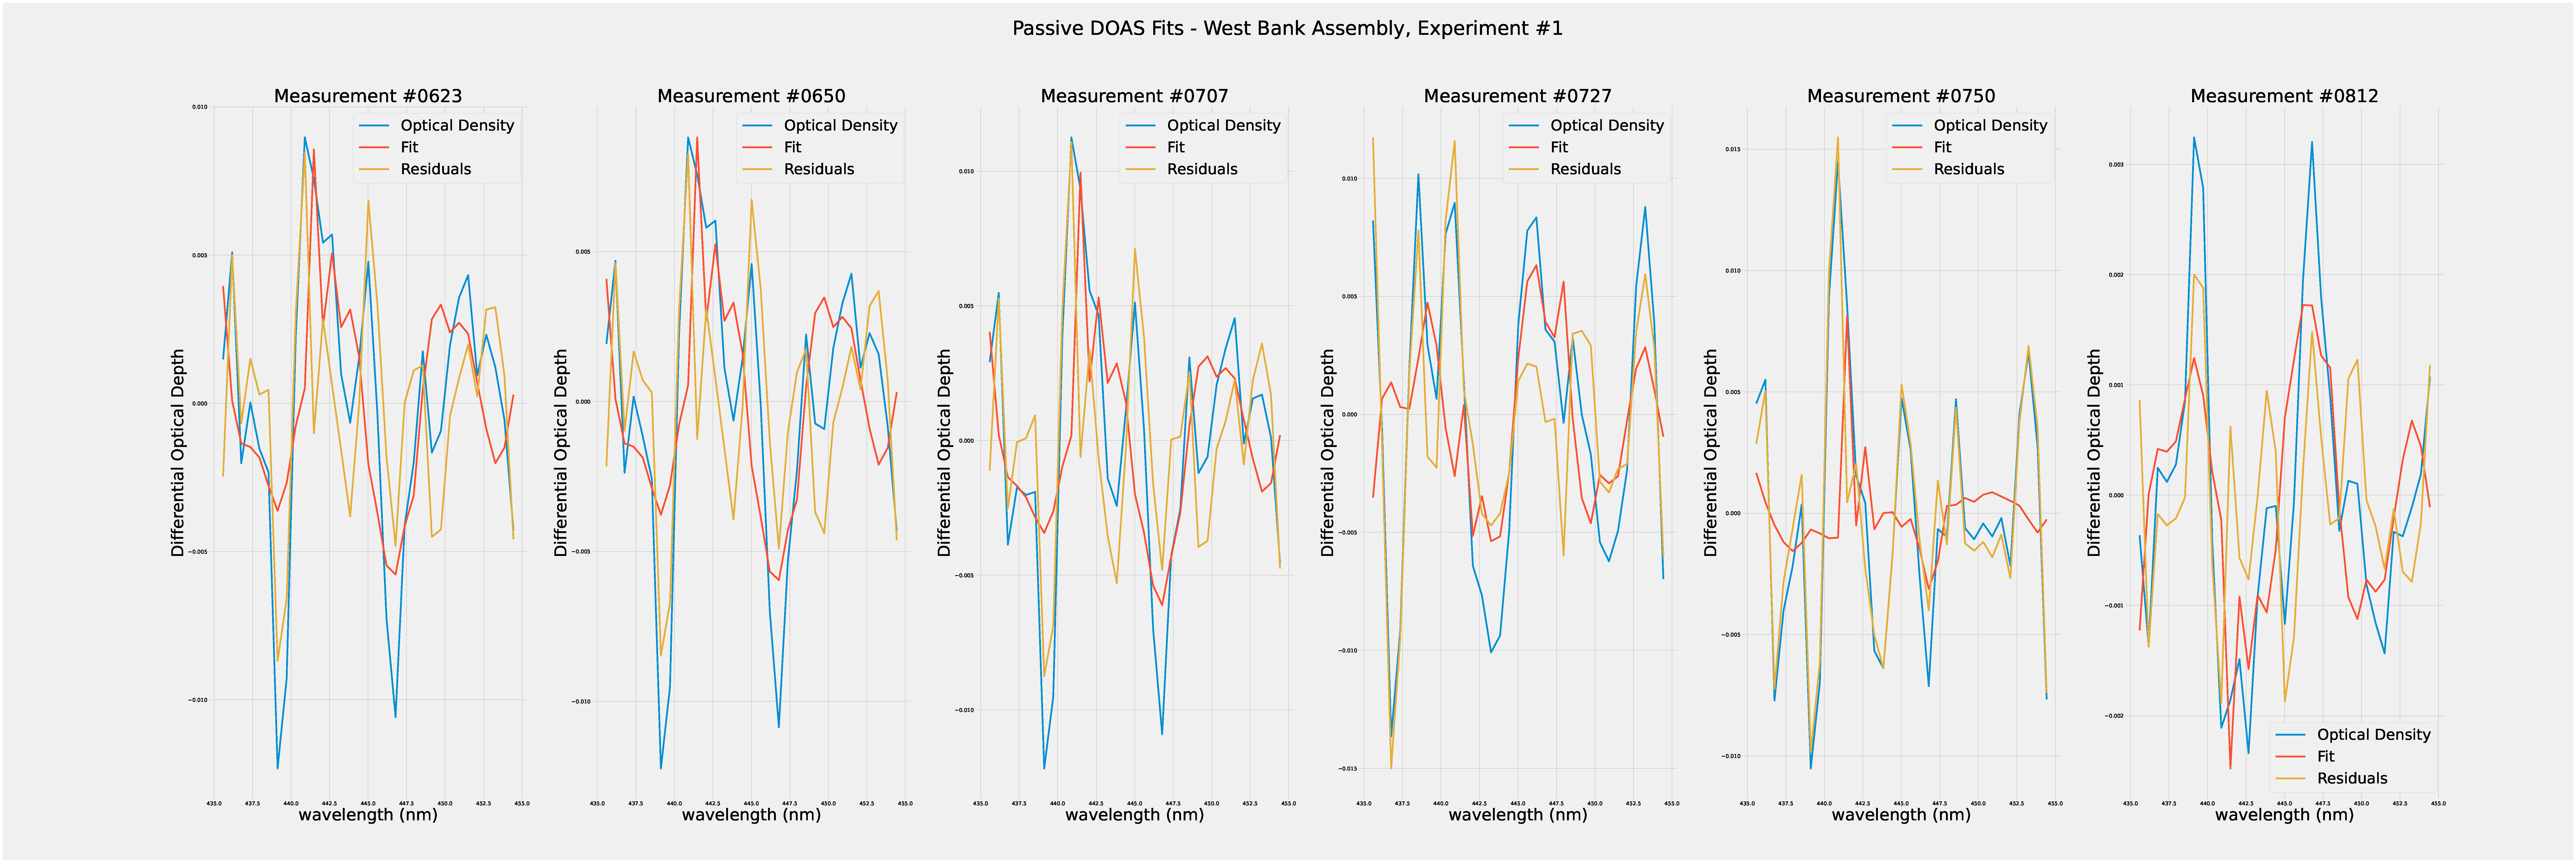
\includegraphics[width = .82\textheight]{img/eps/fit_passive_westbank_exp1.eps}
    \caption{Passive \gls{DOAS} fits for the first run of the
    experiment, collected at the West Bank assembly.}
    \label{fig:exp1_fit_west}
% \end{sidewaysfigure}

% \begin{sidewaysfigure}
    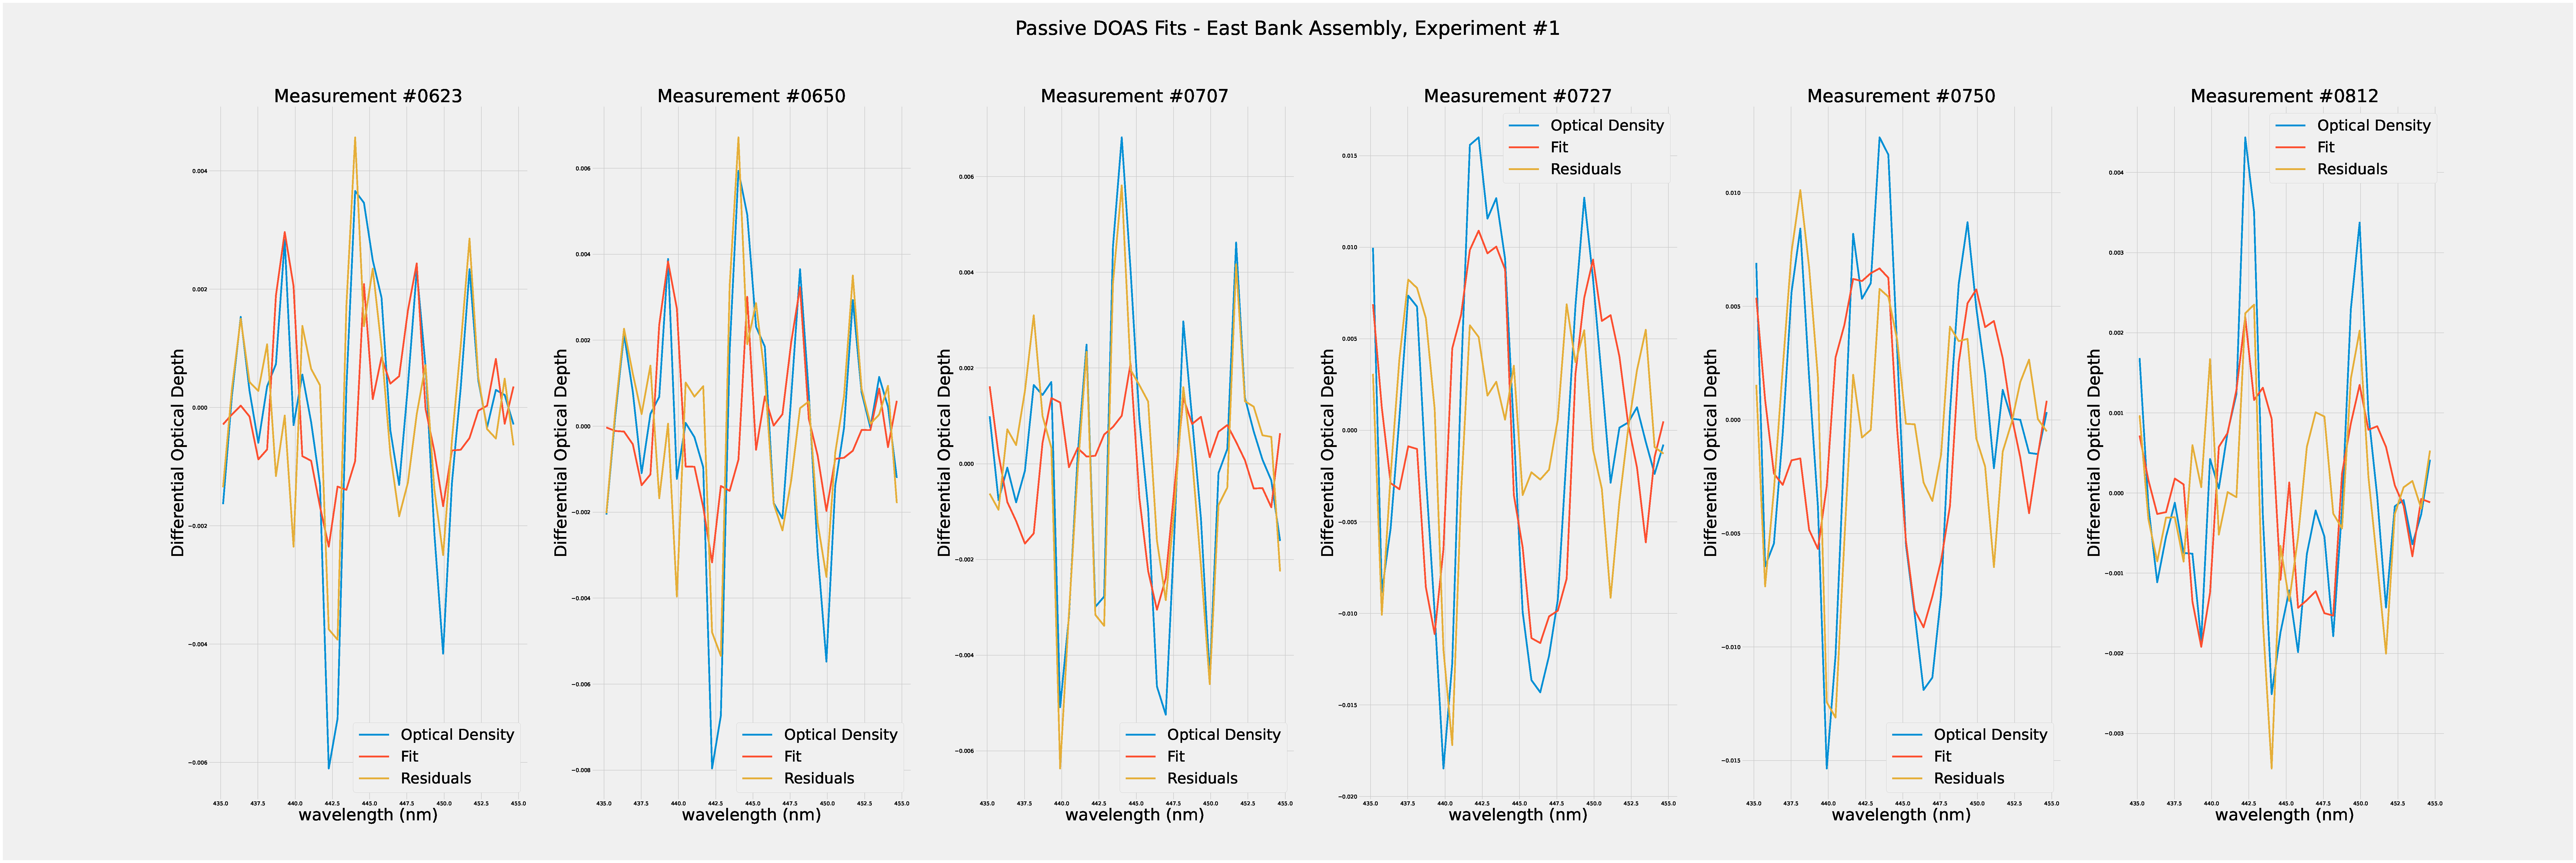
\includegraphics[width=.82\textheight]{img/eps/fit_passive_eastbank_exp1.eps}
    \caption{Passive \gls{DOAS} fits for the first run of the
    experiment, collected at the East Bank assembly.}
    \label{fig:exp1_fit_east}
\end{sidewaysfigure}

\begin{figure}[htpb]
    \centering
    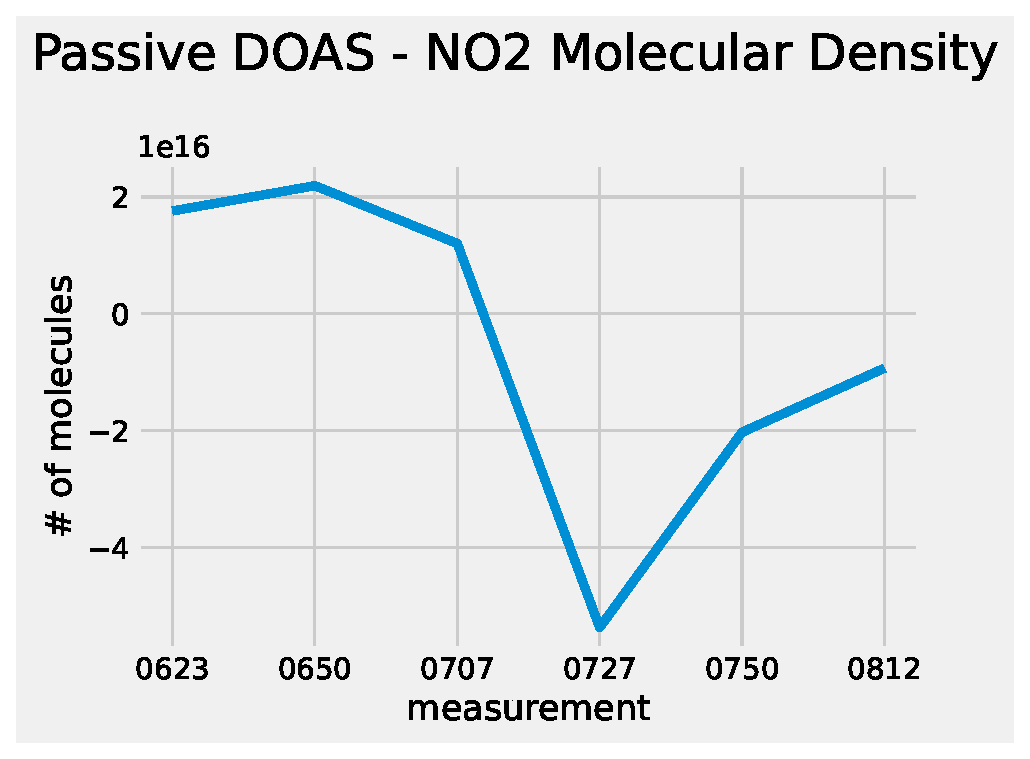
\includegraphics[width=0.8\linewidth]{img/eps/no2_passive_density_exp1.eps}
    \caption{\gls{no2} density values, in number of molecules, for the
    first run of the experiment. Note that the calculated value is the
    subtraction between the density found for the East Bank and the density
    found at the West Bank.}
    \label{fig:exp1_no2_density}
\end{figure}


\begin{table}[htpb]
    \centering
    \caption{Parameters for the DOAS measurements relative to the first
    run of the experiment.}
    \label{tab:doas_parameters_exp1}
    \begin{tabular}{@{}ll@{}}
        \toprule
        \textbf{Parameter}                   & \textbf{Value}    \\
        \midrule
        Analysis Window                      & {[}430, 455{]} nm \\
        \midrule
        Order of Filtering Polynomial        & 2                 \\
        \midrule
        Spectral Resolution                  & 2.4 nm           \\
        \bottomrule
    \end{tabular}
\end{table}

\subsection{Second run}%
\label{sub:second_run}

The second run of this experiment took place on the
23\textsuperscript{rd} of June. The weather was not as perfect as it had
been in the first day, with a few scattered clouds dotting the sky, and
a lot more wind. These clouds were on a completely different azimuth
than the field of study, so they had no influence whatsoever on the
results. The exact spot of the experiment also changed slightly. On the
first run, the East bank assembly was closer to the western limit of the
sanctuary. This run was conducted putting the East bank assembly farther
to the East. This change improved (but also made more difficult) the
artificial light measurements, by providing a better background. It also
improved operational conditions, decreasing human error probability.
This position difference is illustrated in
Figure~\ref{fig:changing_position}.

\begin{figure}[htpb]
    \centering
    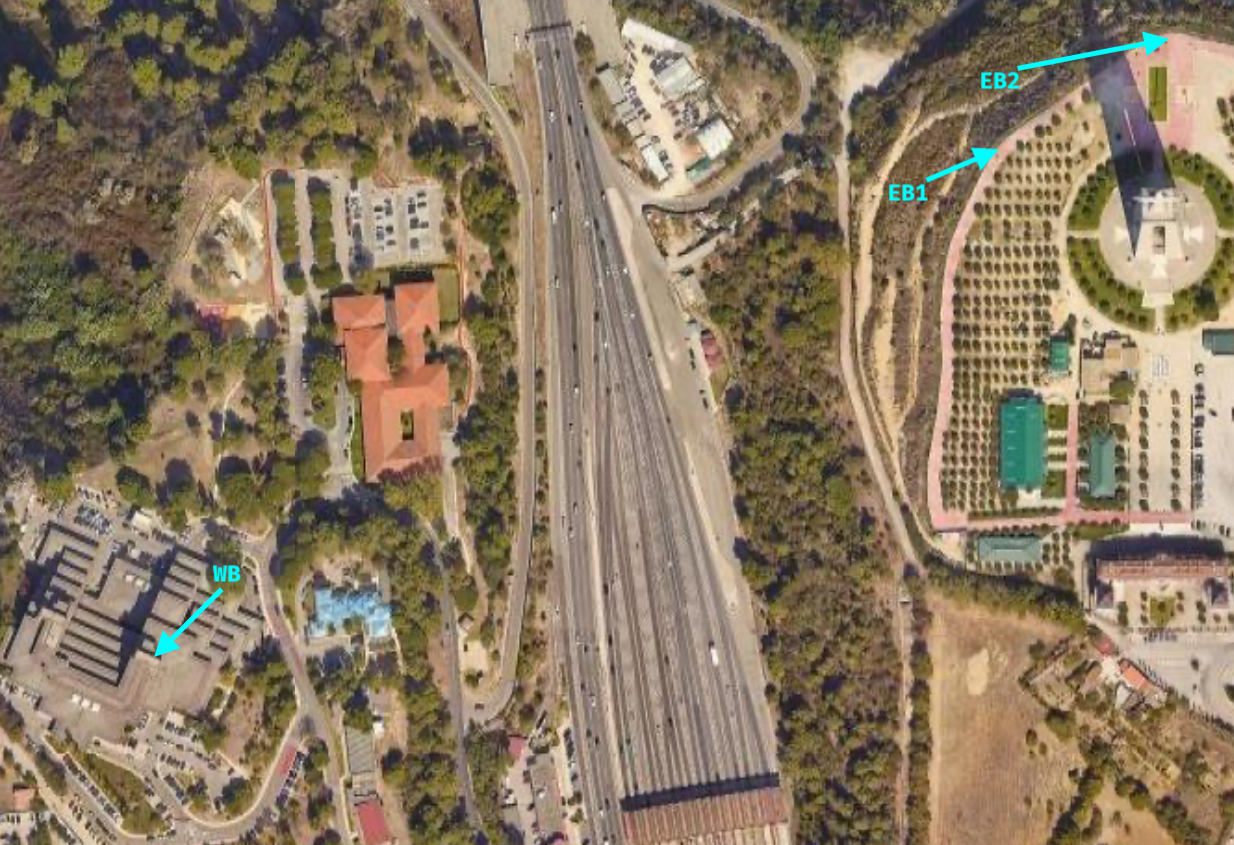
\includegraphics[width=0.8\textwidth]{img/png/eastbank_changed.png}
    \caption{This image, built using Google Maps, illustrates the East
    Bank relocation that took place in the second leg of the experiment.
    The first location is presented as EB1, while the second is naturally
    EB2. The West Bank is also presented for some geographic reference, and
    identified by WB.}
    \label{fig:changing_position}
\end{figure}

Unlike the first run, the second run started without any logistic
hiccup, on time, and we were able to continue measuring until 10:00.
The total number of measurements reached 12. This was slightly under the
16 target measurements, but much better than what we had achieved in the
previous day. Table~\ref{tab:second_run_measurements} contains the time
for each of the performed spectral collections.

\begin{table}[htpb]
    \centering
    \caption{Second run: time of measurements table.}
    \label{tab:second_run_measurements}
    \begin{tabularx}{\textwidth}{@{}lXXXXl@{}}
        \toprule
        \textbf{\#} & \textbf{Active DOAS} & \textbf{Active DOAS Reference} & \textbf{West Bank Passive DOAS} & \textbf{East Bank Passive DOAS} & \textbf{Comments} \\ \midrule
        1           & 06:07                & 05:57                          & 06:14                           & 06:12                           & BAD               \\
        2           & 06:35                & \multirow{2}{*}{06:30}         & 06:40                           & 06:40                           & BAD               \\
        3           & 06:50                &                                & 06:50                           & 07:00                           & BAD               \\
        4           & 07:10                & 07:15                          & 07:00                           & 07:27                           &                   \\
        5           & 07:50                & 07:40                          & 07:10                           & \multirow{3}{*}{07:52}          &                   \\
        6           & 08:08                & 08:03                          & 07:25                           &                                 &                   \\
        7           & 08:18                & 08:21                          & 07:53                           &                                 &                   \\
        8           & 08:35                & 08:30                          & 08:35                           & 08:36                           &                   \\
        9           & 09:00                & 08:53                          & 09:02                           & 09:00                           &                   \\
        10          & 09:45                & 09:50                          & 09:24                           & 09:20                           &                   \\
        11          & 10:00                & 10:05                          & 09:53                           & 09:48                           &                   \\ \bottomrule
    \end{tabularx}
\end{table}

Spectroscopically, the collected data were of good quality.
Unfortunately, in terms of the experiment itself, some had to be
discarded. This is chiefly true with regard to the artificial light
portion of the experiment. With the change in position described in the
previous paragraph, the light came to fill a much smaller visual slice
than in the first run. This meant that it was much more difficult to
pick up the torch with the telescope on the West bank. Although I have
tried to align both telescopes in order to only capture the light that I
was interested in, in more than one occasion, this alignment was
(probably by the wind) destroyed. Since the light was so small in
comparison with the field of vision, the final resulting spectrum is one
of the background instead of the torch. In the end, only 8 measurements
were viable. Analytical parameters are found in
Table~\ref{tab:doas_parameters}. Figure~\ref{fig:active_densities} and
Figures~\ref{fig:passive_densities} are plots of the measured
concentration of \gls{no2}. Figures~\ref{fig:fit_active},
Figure~\ref{fig:fit_passive_back} and Figure~\ref{fig:fit_passive_front}
are the plots showing the actual \gls{DOAS} fits.

\begin{table}[htpb]
    \centering
    \caption{Parameters for the DOAS measurements relative to the second
    run of the experiment.}
    \label{tab:doas_parameters}
    \begin{tabular}{@{}ll@{}}
        \toprule
        \textbf{Parameter}                   & \textbf{Value}    \\
        \midrule
        Analysis Window - Active Experiment  & {[}400, 450{]} nm \\
        \midrule
        Analysis Window - Passive Experiment & {[}430, 455{]} nm \\
        \midrule
        Order of Filtering Polynomial        & 2                 \\
        \midrule
        Spectral Resolution                  & 2.4 nm           \\
        \bottomrule
    \end{tabular}
\end{table}

\begin{figure}[htpb]
    \begin{minipage}[t]{.45\textwidth}
        \centering
        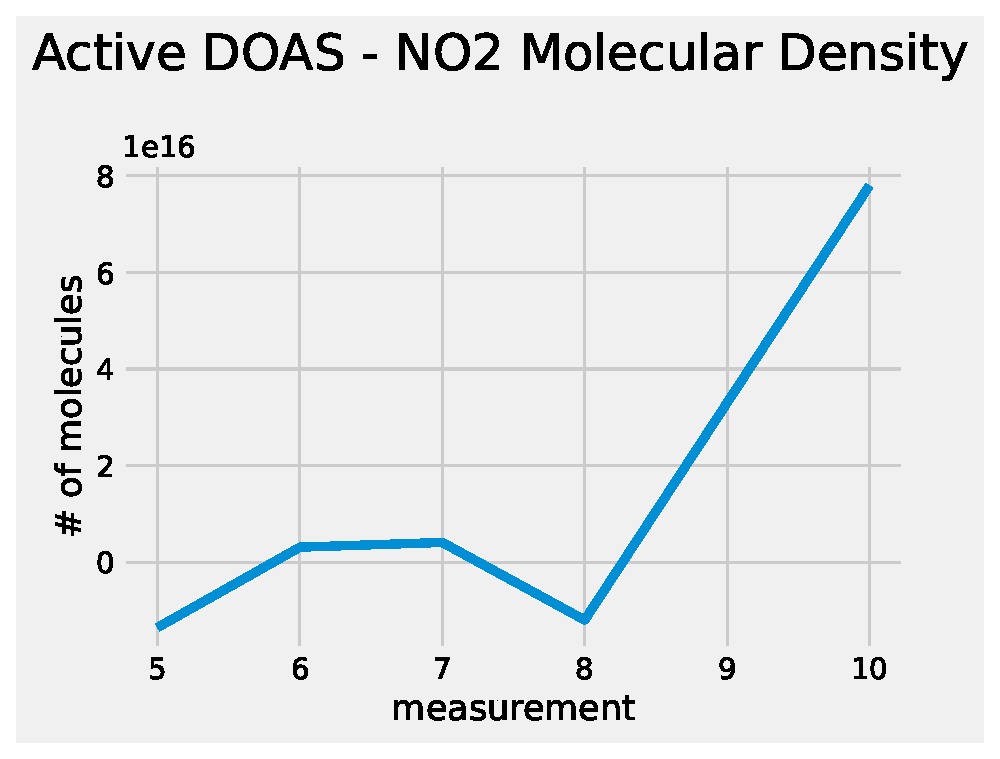
\includegraphics[width=\linewidth]{img/eps/no2_active_density.eps}
        \caption{Active \gls{DOAS} molecular density for \gls{no2}, varying
        with the measurement number.}
        \label{fig:active_densities}
    \end{minipage}
    \hfill
    \begin{minipage}[t]{.45\textwidth}
        \centering
        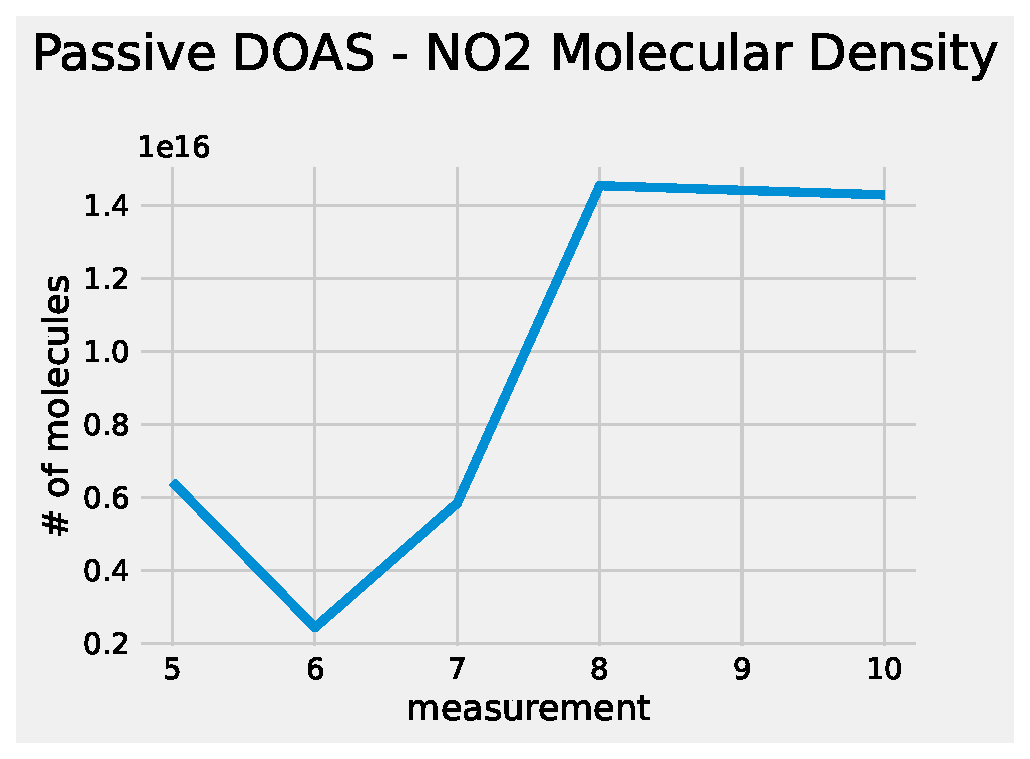
\includegraphics[width=\linewidth]{img/eps/no2_passive_density.eps}
        \caption{Passive \gls{DOAS} molecular density for \gls{no2}, varying
        with the measurement number. Note that this is the difference
        between the density obtained at the two experiment assemblies, as per
        hypothesis 2 (see~\ref{sec:second_hypothesis}).}
        \label{fig:passive_densities}
    \end{minipage}
\end{figure}

\begin{sidewaysfigure}[htpb]
    \centering
    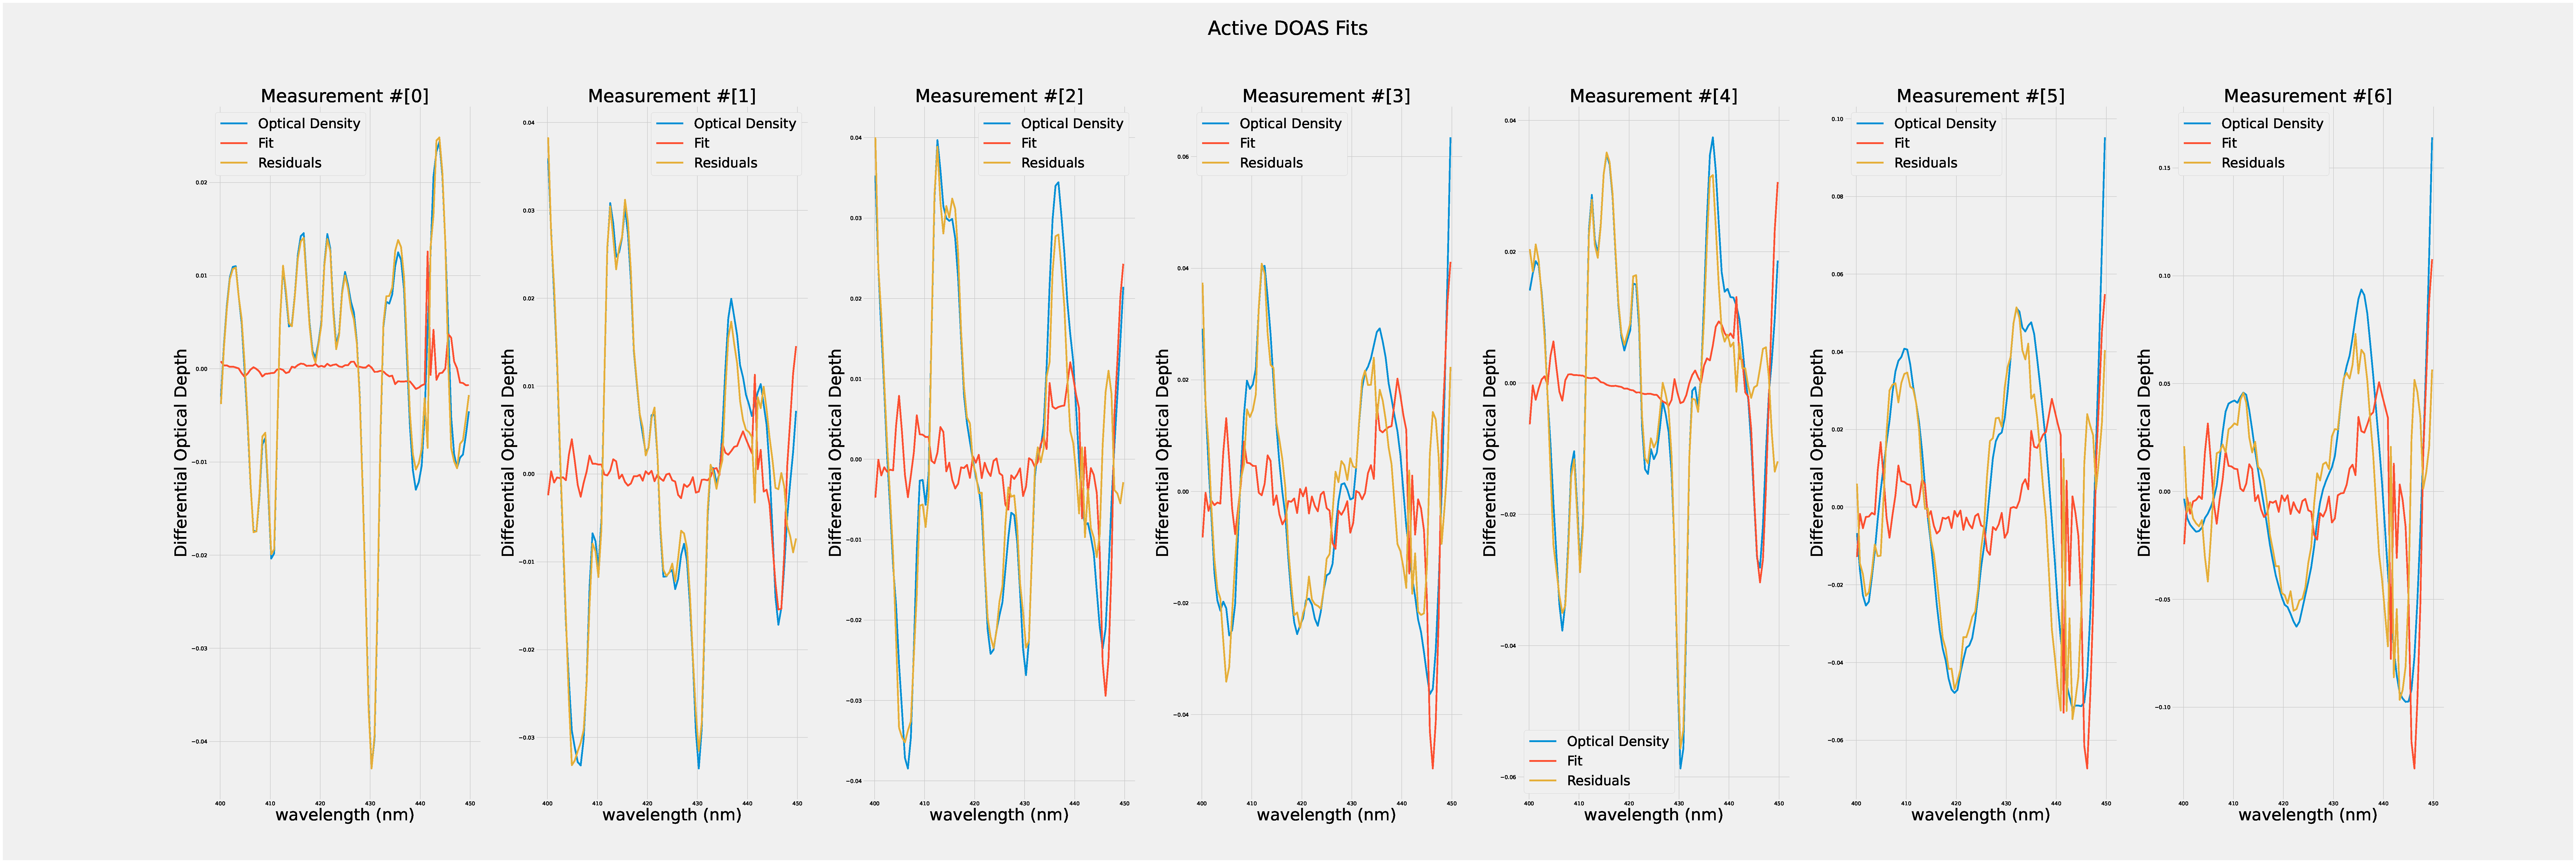
\includegraphics[width=\textheight]{img/eps/fit_active.eps}
    \caption{Active \gls{DOAS} fit results. Each plot corresponds to one
    measurement moment.}
    \label{fig:fit_active}
\end{sidewaysfigure}

\begin{sidewaysfigure}[htpb]
    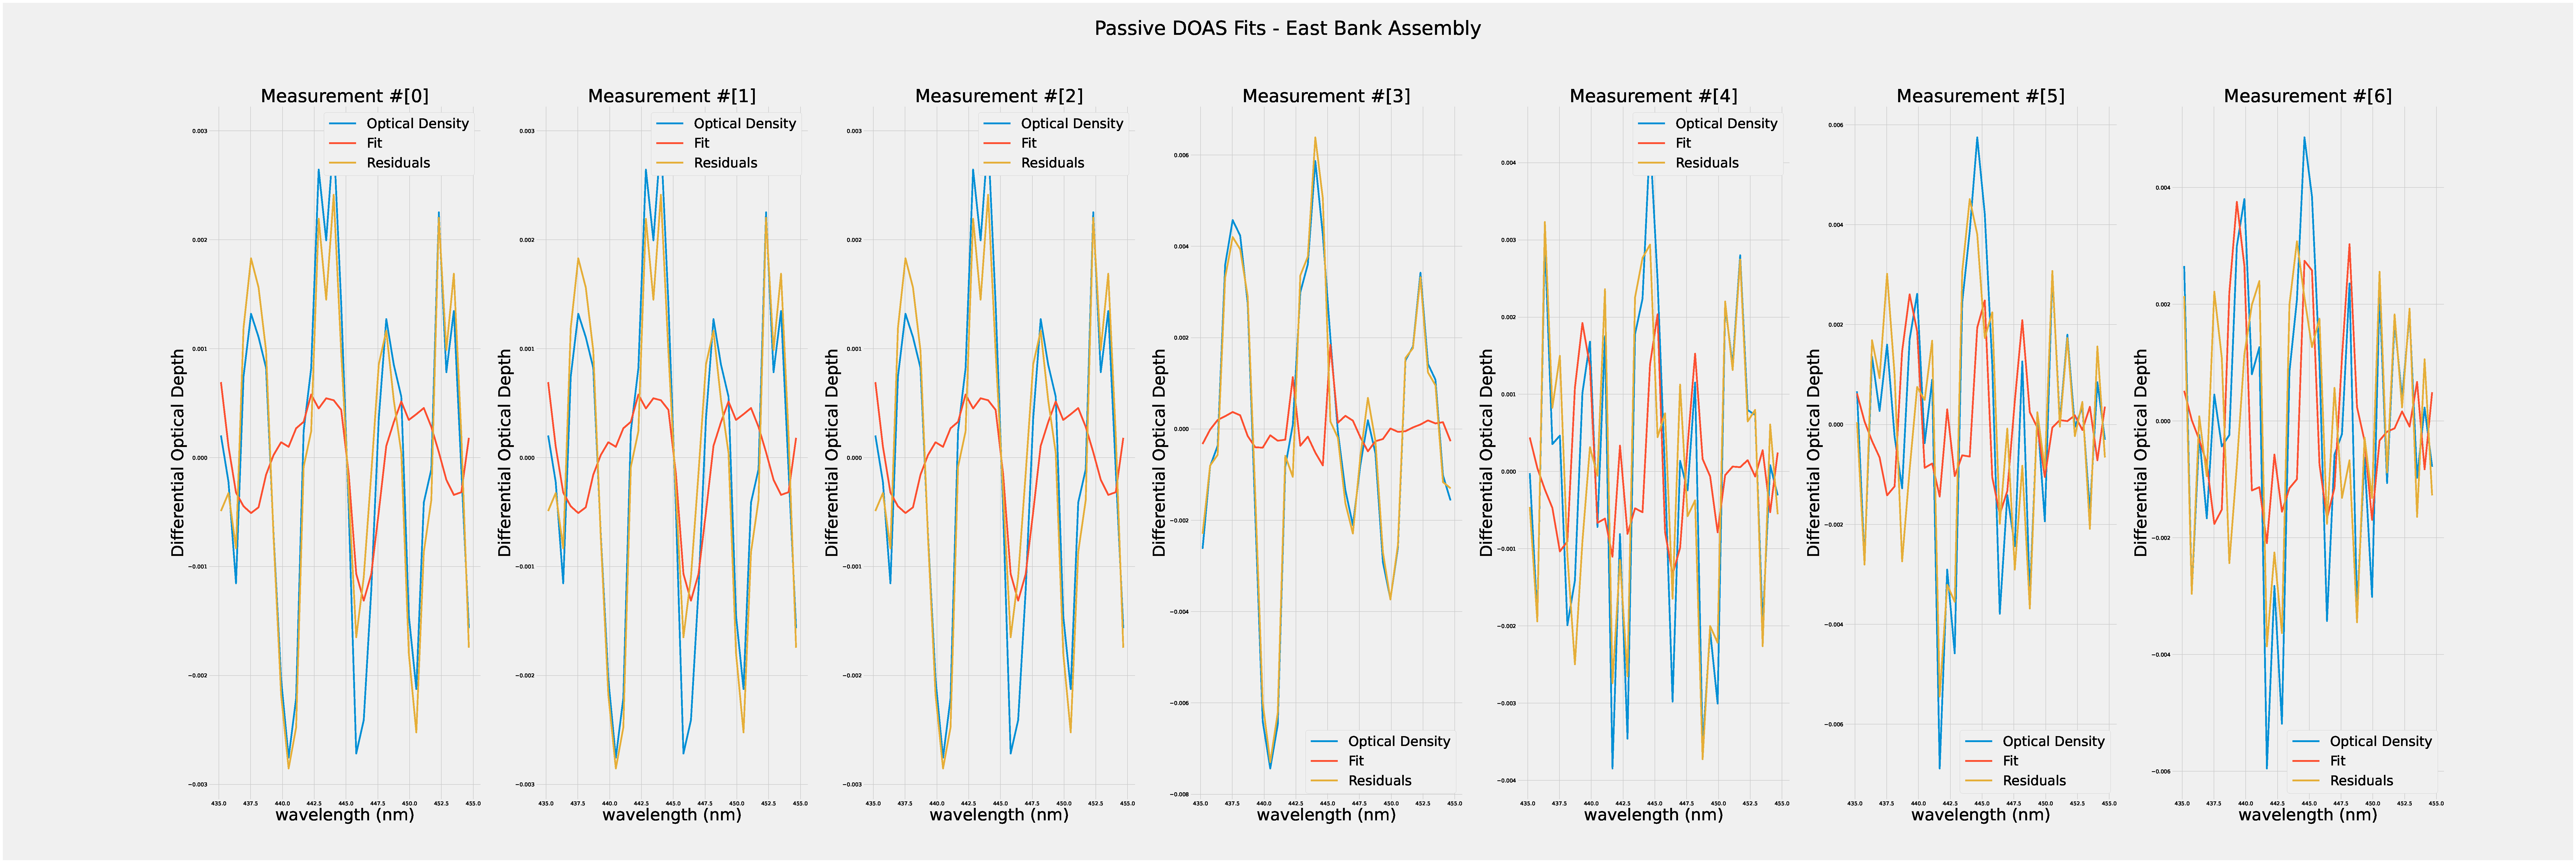
\includegraphics[width=.82\textheight]{img/eps/fit_passive_back.eps}
    \caption{Passive \gls{DOAS} fit results, from the system on the East
    Bank. Each plot corresponds to one measurement moment.}
    \label{fig:fit_passive_back}
    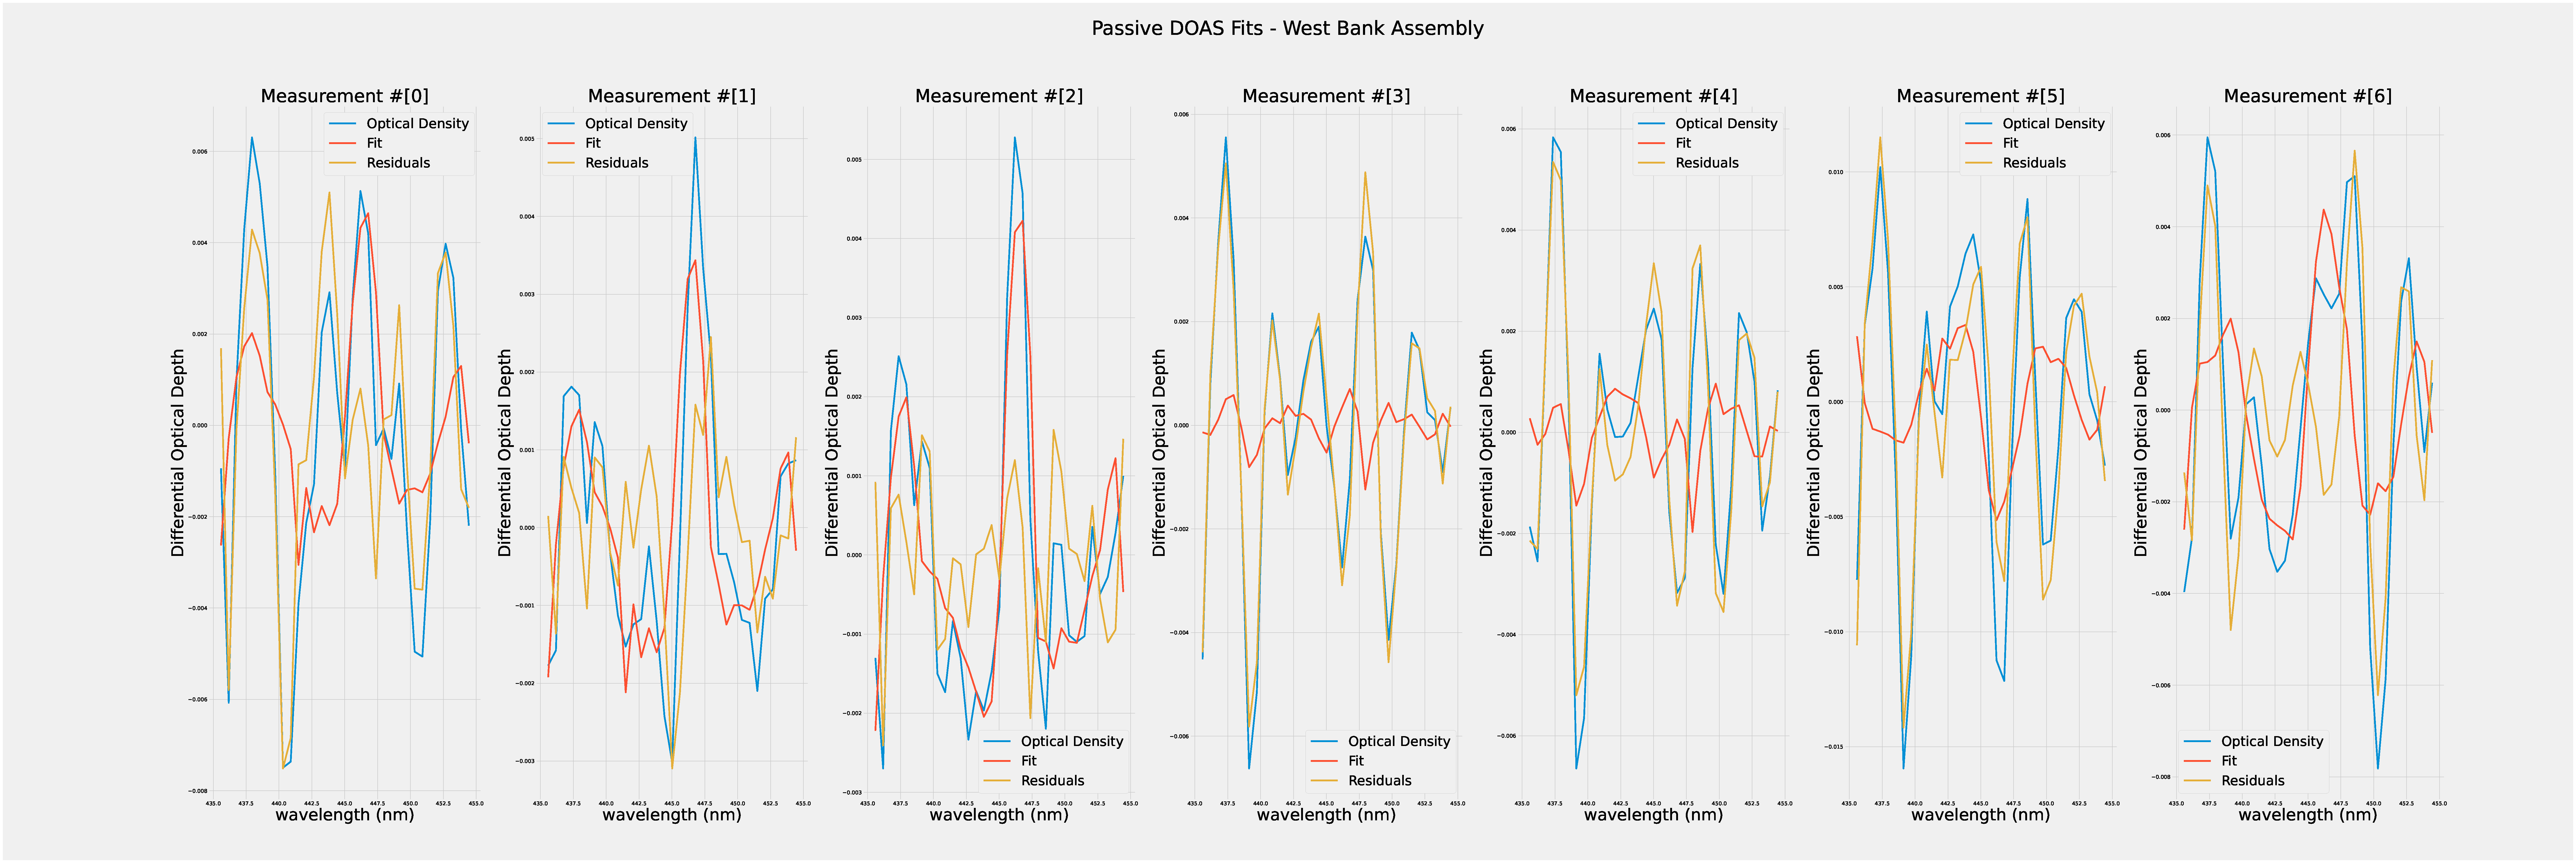
\includegraphics[width=.82\textheight]{img/eps/fit_passive_front.eps}
    \caption{Passive \gls{DOAS} fit results, from the system on the West
    Bank. Each plot corresponds to one measurement moment.}
    \label{fig:fit_passive_front}
\end{sidewaysfigure}

\subsection{Data Processing}%
\label{sub:data_processing}

While the rest of this section is dedicated to the gathering of spectral
data and even the results that it returns, it is important to mention
and to provide a (brief, high level) description of what is being done
to said data.

AvaSoft, Avantes' spectrometer handling software application, allows one
to store collected data in several formats. Most of these formats are
binary in nature. These are more compact in terms of occupied disk space
and are commonly used in this kind of application because spectra are
most likely being collected for later processing through another
computer program. However, they are not good if one needs to quickly
check if the data are being correctly gathered or to see if there was
any kind of operation error in the collection process, since they are
completely unintelligible for humans. For this purpose, Avantes make the
Avantes \gls{ascii} file format available. This is, as its name might
imply, an \gls{ascii} formatted file that can be quickly inspected by
anoyone that can read the English language and understand the Latin
characters. The files have a particular structure which is illustrated
by Figure~\ref{fig:avantesASCIIFile}.

\begin{figure}[htpb]
    \centering
    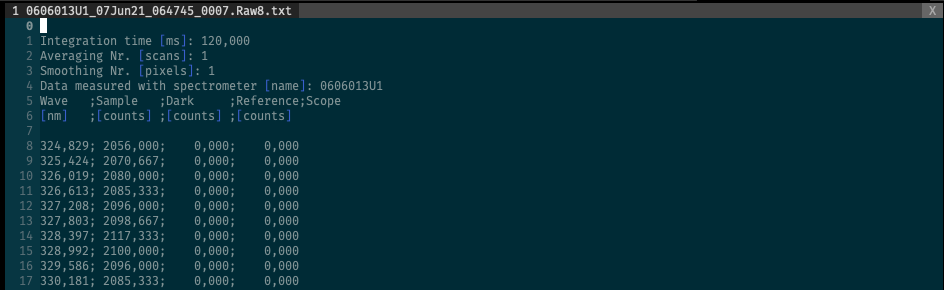
\includegraphics[width=\linewidth]{img/png/avantes_ascii.png}
    \caption{The Avantes ASCII file format. This is a screenshot of a
        file of this type opened in the VIM text editor. Note its
        particular structure, around which the file / folder parsing
        objects described by Figure~\ref{fig:avantesASCIIFileLoader} and
        Figure~\ref{fig:avantesASCIIFolder} are constructed.}
        \label{fig:avantesASCIIFile}
\end{figure}

Some light string parsing operations are the compromise that is required
to use this kind of file format in analytical software. In the case of
this thesis' application, the files are opened and parsed using an
\gls{oop} approach that takes advantage of the organisational structure
of the several files involved in the process. Each file originates an
AvantesASCII object, which loads the data, parses its values and stores
them in a Pandas DataFrame internal object~\footnote{Pandas is a data
processing library used in Python that provides a very efficient way to
access and manipulate tabular data by leveraging the use of C code
through Python commands.}. For each folder that contains this kind of
file, the parsing library creates an AvantesASCIIFolder object, which
loads all files inside that folder and runs global data operations such
as summation and integration-time-normalisation. A general schematic of
this approach is provided in Figure~\ref{fig:data_processing_general},
while a flowchart for the file loading routine is presented in
Figure~\ref{fig:avantesASCIIFileLoader} and the folder loading process
is illustrated by Figure~\ref{fig:avantesASCIIFolder}.

\begin{figure}[htpb]
    \centering
    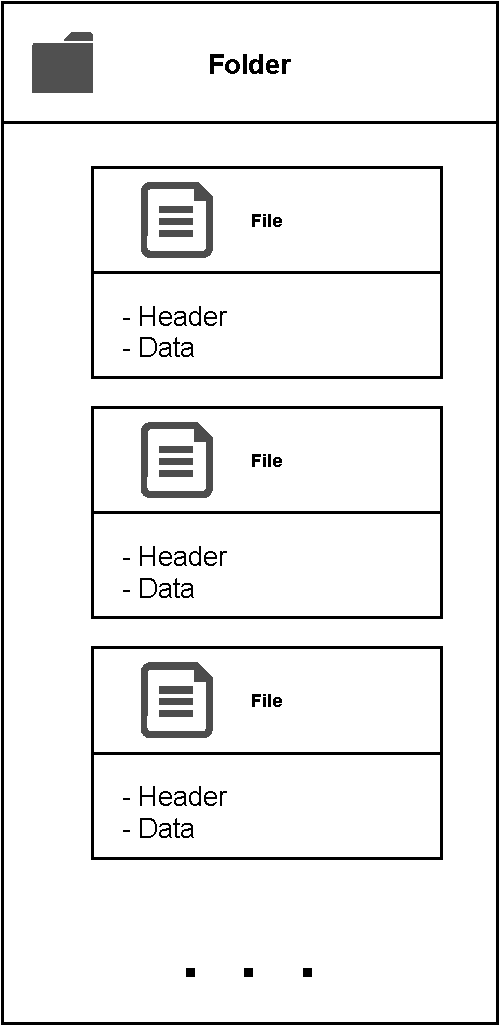
\includegraphics[width=0.3\linewidth]{img/pdf/data_processing_general.pdf}
    \caption{The Data processing. The \gls{oop} approach that was taken
    attempts to take advantage of the organisational structure of the
    spectral data, by modelling it into Python objects.}
    \label{fig:data_processing_general}
\end{figure}

\begin{figure}[htpb]
    \begin{minipage}{.45\textwidth}
        \centering
        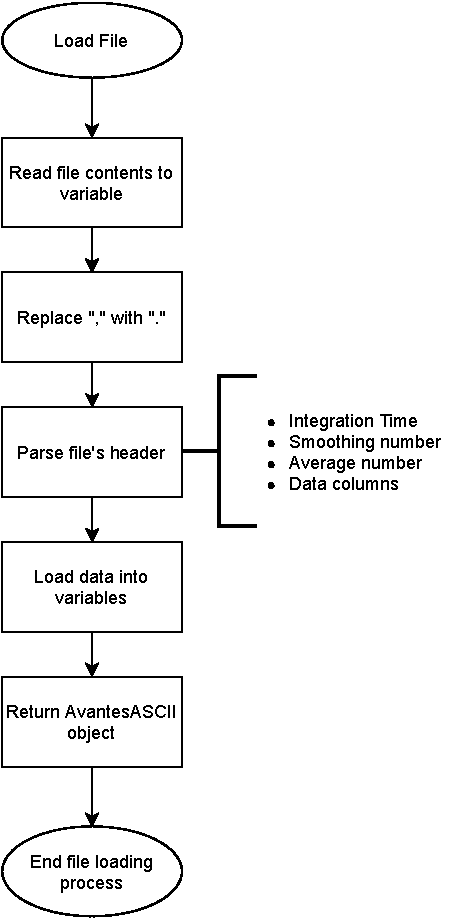
\includegraphics[width=0.7\linewidth]{img/pdf/file_loading.pdf}
        \caption{The file loading process. An Avantes ASCII file originates
        an AvantesASCII object, which besides a series of string-parsing
        operations stores the data in a Pandas DataFrame, for easy access and
        control.}
        \label{fig:avantesASCIIFileLoader}
    \end{minipage}
    \hfill
    \begin{minipage}{.45\textwidth}
        \centering
        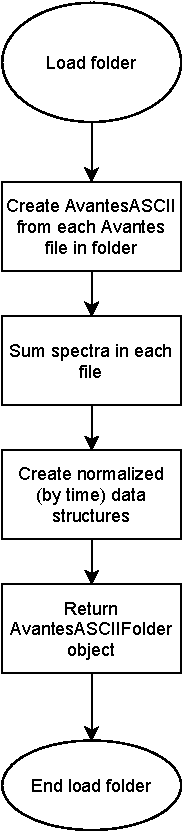
\includegraphics[width=0.3\linewidth]{img/pdf/folder_loading.pdf}
        \caption{The folder loading process. Each folder can have many
        files. The way in which the data is gathered (described in
        Subsection~\ref{sub:experiment_first_run}) requires some global
        operations performed on groups of files, like summation and
        normalisation (with reference to the integration time). The
        AvantesASCIIFolder object provides such operations.}
        \label{fig:avantesASCIIFolder}
    \end{minipage}
\end{figure}

\subsection{The DOAS Library}%
\label{sub:the_doas_library}

The \gls{DOAS} software library is a Python package developed
specifically for this thesis data processing operations. It was, as
other components, designed using an \gls{oop} approach and following the
SOLID principles of \acrlong{oop}. This piece of software was written in
response to the initial research that I undertook and that returned no
usable results in terms of modular, compact Python libraries for
\gls{DOAS} applications, that I could use in my work. It is, as far as I
know,  the only \gls{DOAS} solving application with this kind of
structure.

The library (\gls{uml} diagram presented in
Figure~\ref{fig:doas_library}) models a \gls{DOAS} application through
the instrumentation lens. A \gls{DOAS} application is always
parametrised through its spectrometer's physical features and
limitations, which in turn determine the structure of the analysed
spectral data, and even the differential cross sections of the trace
gases that are to be studied. Of course, this library is much more
limited in its capabilities than some specific programs that have become
commonplace in this kind of application, such as
QDOAS~\cite{Danckaert2015}, but the fact that it can be operated through
a Python program and that one can manipulate the data through such tools
as Pandas DataFrames more than make up for this lack. Moreover, since it
is in effect a software library, it is also as flexible as one is
willing to expand it.

\begin{figure}[htpb]
    \centering
    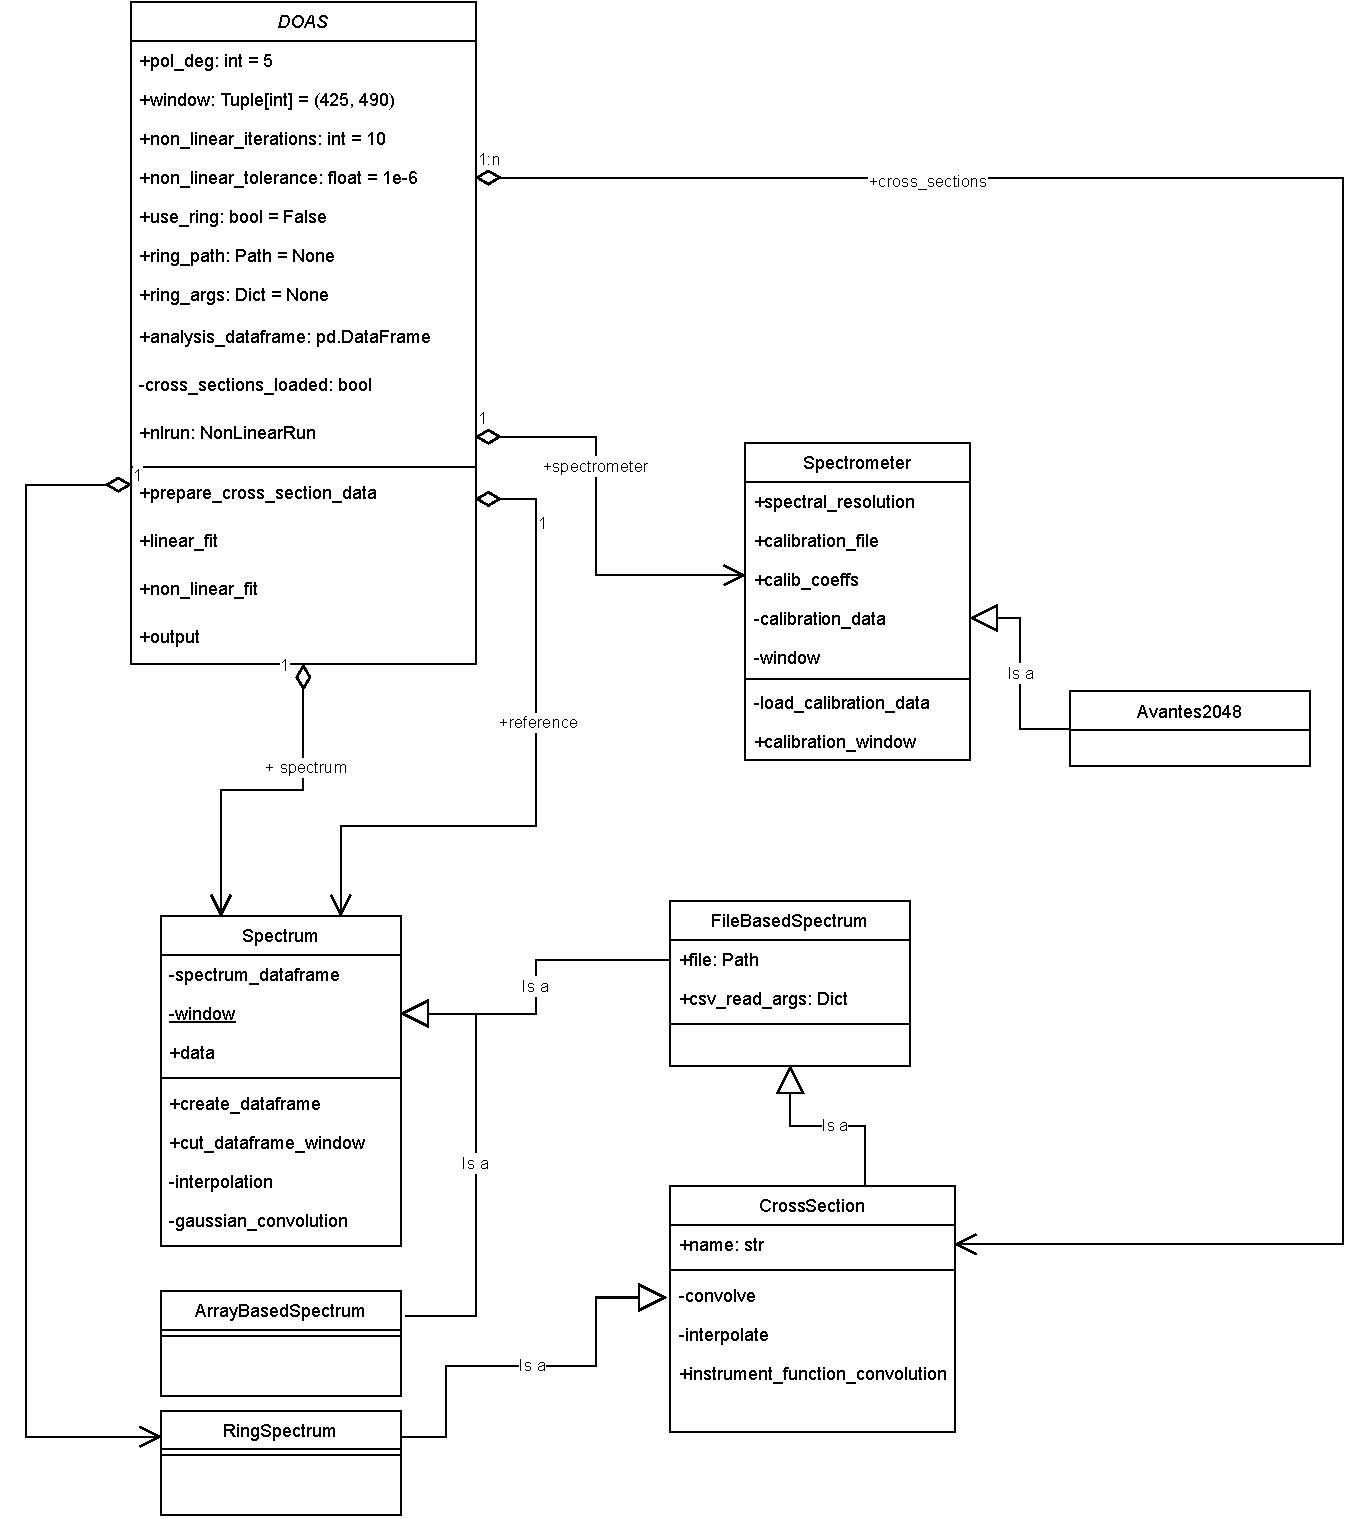
\includegraphics[width=0.8\linewidth]{img/pdf/uml_doas.pdf}
    \caption{UML diagram for the \gls{DOAS} library. The \gls{oop}
    approach that was followed allows for an instrument-oriented
    experiment parametrisation, which is not available in any other
    software}
    \label{fig:doas_library}
\end{figure}

An important side note that attests to this library's relevance is that
it has been fully integrated in FutureCompta's Bee2Fire software, with
further developments being conducted through this team's efforts. This
is the first commercially applicable result provided by the work in this
thesis.
